\documentclass[12pt,a4paper]{article}
\usepackage{physics}
\usepackage{amssymb}
\usepackage{subcaption}
\usepackage{colortbl}
\newcommand{\activity}{Activity 7 -- Image Segmentation}
\input{spp.dat}

\begin{document}

\title{\TitleFont \activity}
\author[ ]{\textbf{Kenneth V. Domingo} \\
2015--03116 \\
App Physics 186, 1\textsuperscript{st} Semester, A.Y. 2019--20}
\affil[ ]{\corremail{kvdomingo@up.edu.ph} }

\maketitle
\thispagestyle{titlestyle}

\section*{Grayscale Segmentation}
As a warmup for this activity, let's start with a grayscale image of a check (Fig. \ref{fig:check}). First we'll try to segment the text manually. Looking at its histogram (Fig. \ref{fig:check-hist}), we can see that there is a high concentration of pixel values around 200, which corresponds to the background. For now, 125 looks like a good threshold value, so we'll choose to display only pixel values less than 125. The output (Fig. \ref{fig:check-thres}) shows that we have a decent segmentation, and we can choose to leave it at that. However, we don't want to just randomly pick a threshold that looks ``good enough'', so we'll try a slightly more elaborate method. I recall that when I was applying for IPL, I read and presented a paper, whose very rough gist is that it made use of Otsu's method of thresholding to detect malaria in red blood cells \cite{malaria}. Otsu's method searches exhaustively for the threshold value that minimizes the intra-class variance \cite{otsu} and works most effectively if the gray histogram is bimodal. Looking back at Fig. \ref{fig:check-hist}, we can see two general peaks: one about 200 and another about 150, so we expect that Otsu's method will work just fine. Applying Otsu's method yields a threshold value of 146, and the result is shown in Fig. \ref{fig:check-otsu}. Aside from the text being much clearer, we won't see much difference because it's quite a simple image. We'll check again later on to see how well this method fares with color images.

\begin{figure}[htb]
	\centering
	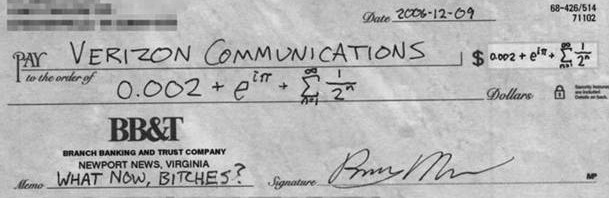
\includegraphics[width=0.75\textwidth]{grayscale_check.jpg}
	\caption{Grayscale image of a check.}
	\label{fig:check}
\end{figure}

\begin{figure}[htb]
	\centering
	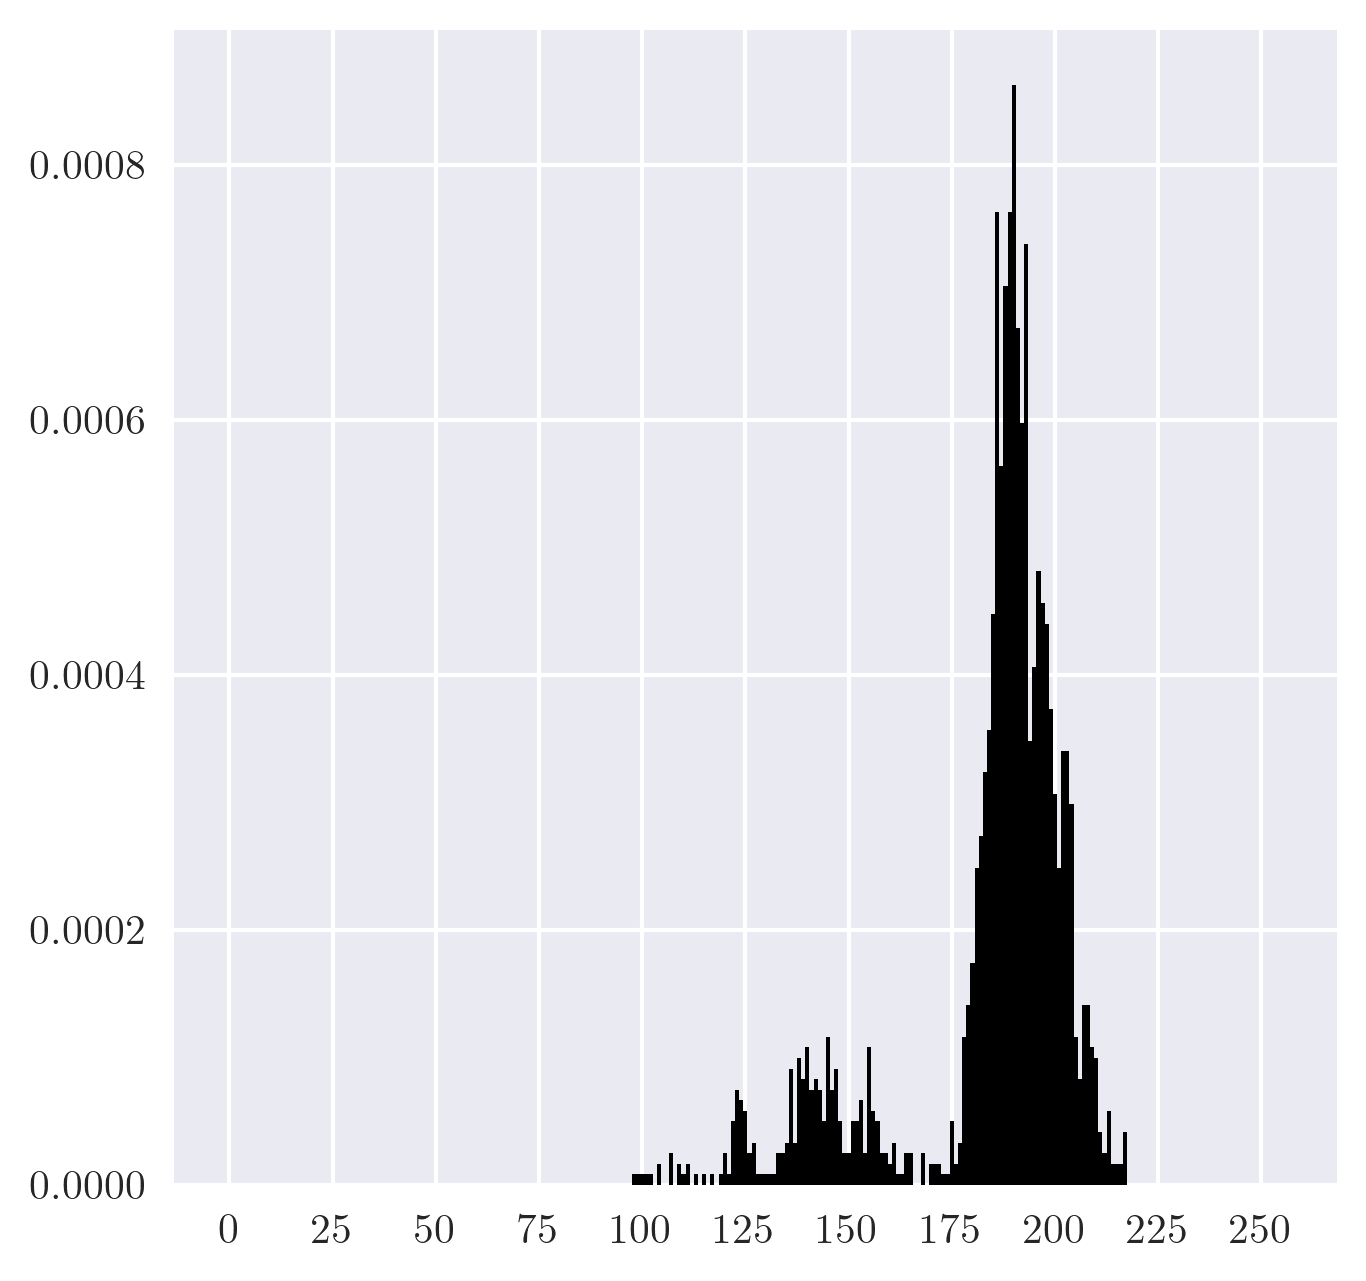
\includegraphics[width=0.5\textwidth]{check_hist.png}
	\caption{Histogram of the check.}
	\label{fig:check-hist}
\end{figure}

\begin{figure}[htb]
	\centering
	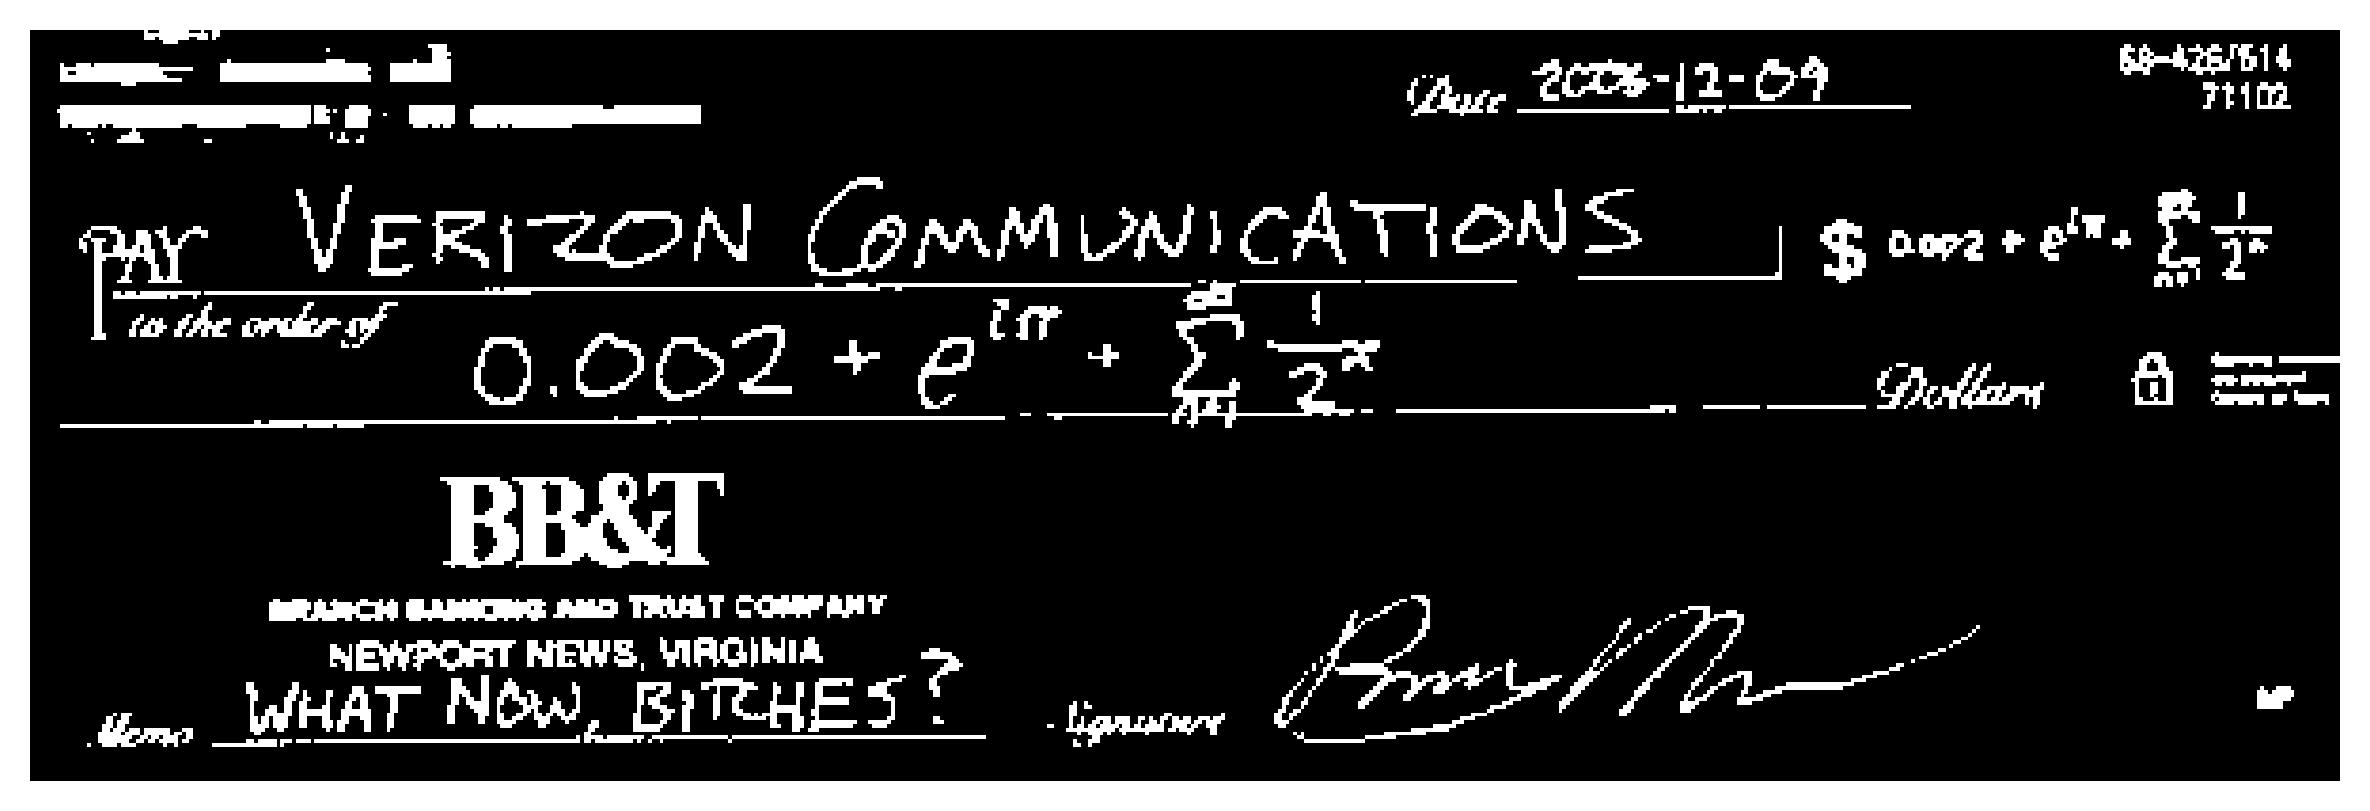
\includegraphics[width=0.75\textwidth]{check_thres125.png}
	\caption{Segmented check with a threshold of 125.}
	\label{fig:check-thres}
\end{figure}

\begin{figure}[htb]
	\centering
	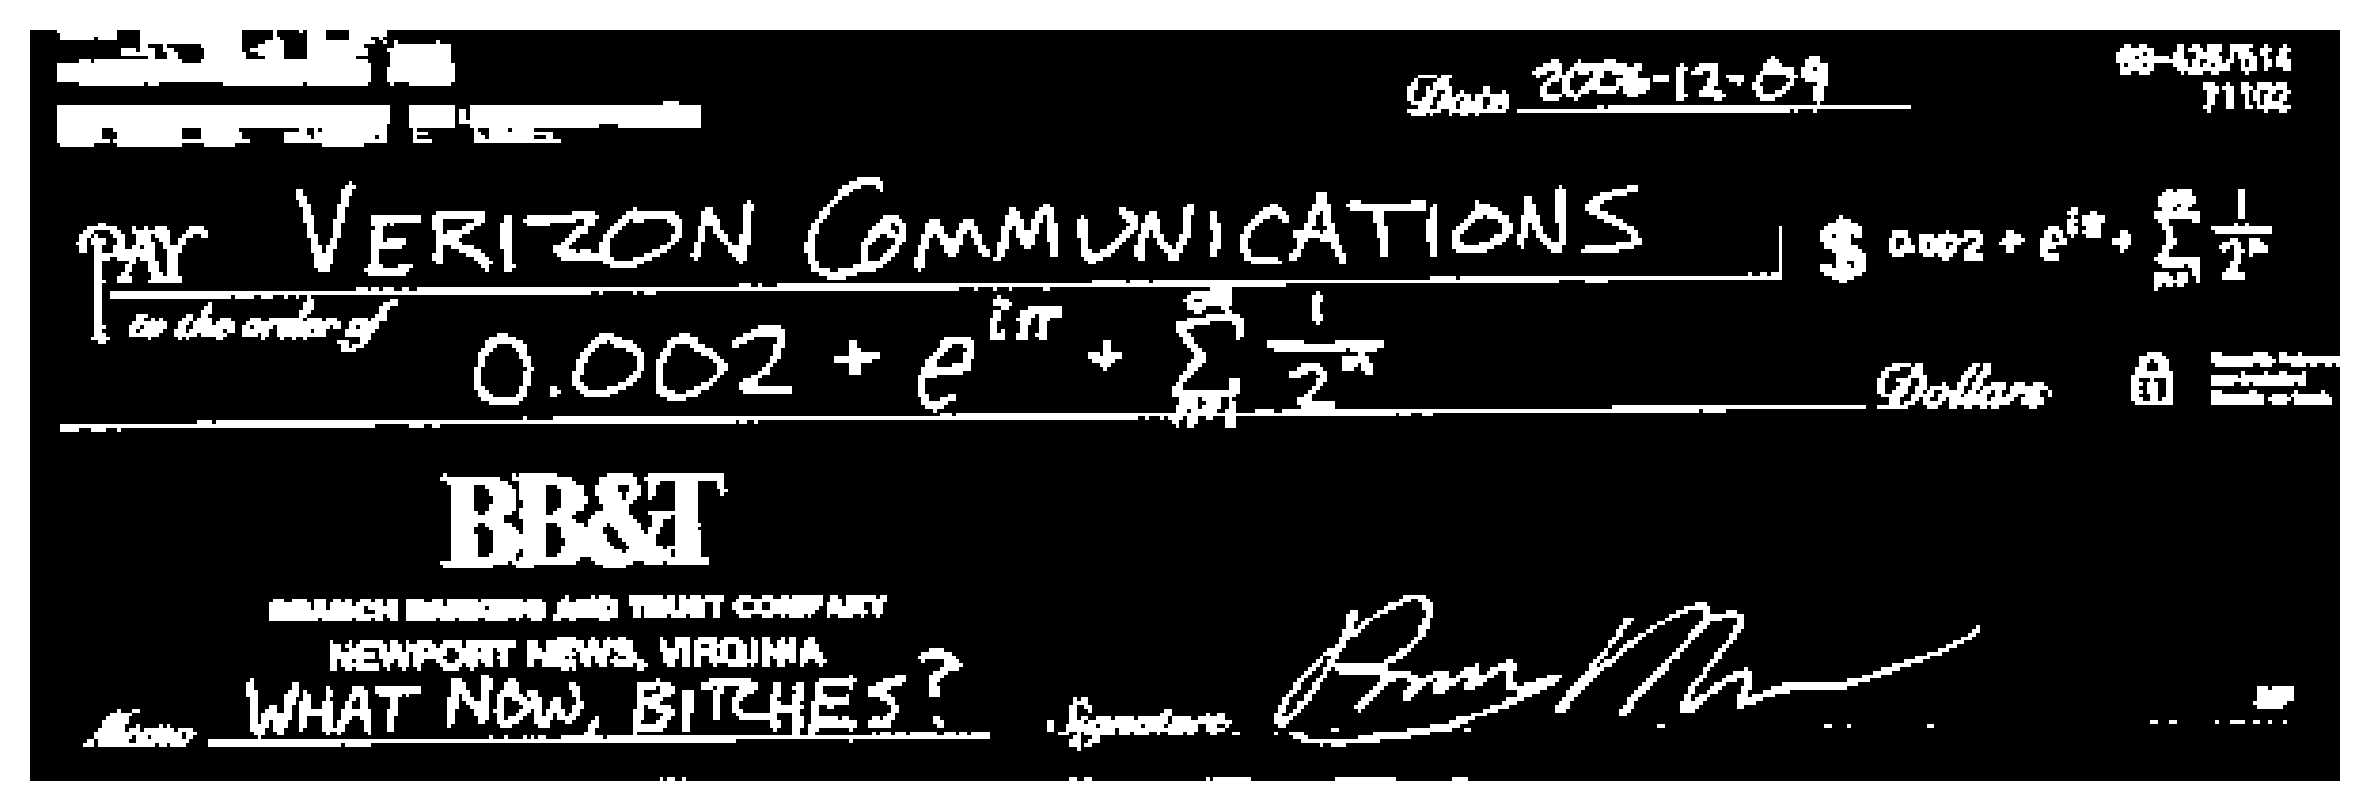
\includegraphics[width=0.75\textwidth]{check_otsu.png}
	\caption{Segmented check using Otsu's method.}
	\label{fig:check-otsu}
\end{figure}

\clearpage
\section*{Color Segmentation}
\setcounter{section}{1}

For the testing phase of this section, I first used the image of a Macbeth ColorChecker to verify final segmentation outputs and histograms. The image is first converted to NCC space via \cite{soriano}

\begin{align}
	I &= R + G + B \label{eq:ncc} \\
	r &= \frac{R}{I} \nonumber \\
	g &= \frac{G}{I} \nonumber
\end{align}

\subsection{Parametric segmentation}
The means $\mu_r, \mu_g$ and standard deviations $\sigma_r, \sigma_g$ of the $r$ and $g$ channels of the region of interest (ROI) are computed, and the probabilities that the original image $r,g$ values $x$ belong to the ROI are computed via

\begin{equation}\label{eq:probability}
	\Pr(x) = \frac{1}{\sqrt{2\pi\sigma^2}} \exp[-\frac{(x - \mu_r)^2}{2\sigma_r^2}]
\end{equation}

\noindent assuming that the $r$ and $g$ pixel values are normally distributed. The final segmented image is produced by obtaining the joint probability $\Pr(r) \times \Pr(g)$.

\subsection{Non-parametric segmentation}
The ROI $r,g$ values are binned into $32 \times 32$ unique combinations of $r,g$ values to form a 2D histogram. This will serve as the lookup table (LUT) for segmenting the original image. The backprojection portion of the code was formulated with some help from \cite{barteezy}.

\subsection{Implementation: Macbeth ColorChecker}
For the first trial, the region of interest is the red patch from the Macbeth ColorChecker. The original image along with outputs from the two algorithms are shown in Figs. \ref{fig:macbeth-red}--\ref{fig:macbeth-black}.

\begin{figure}[htb]
	\centering
	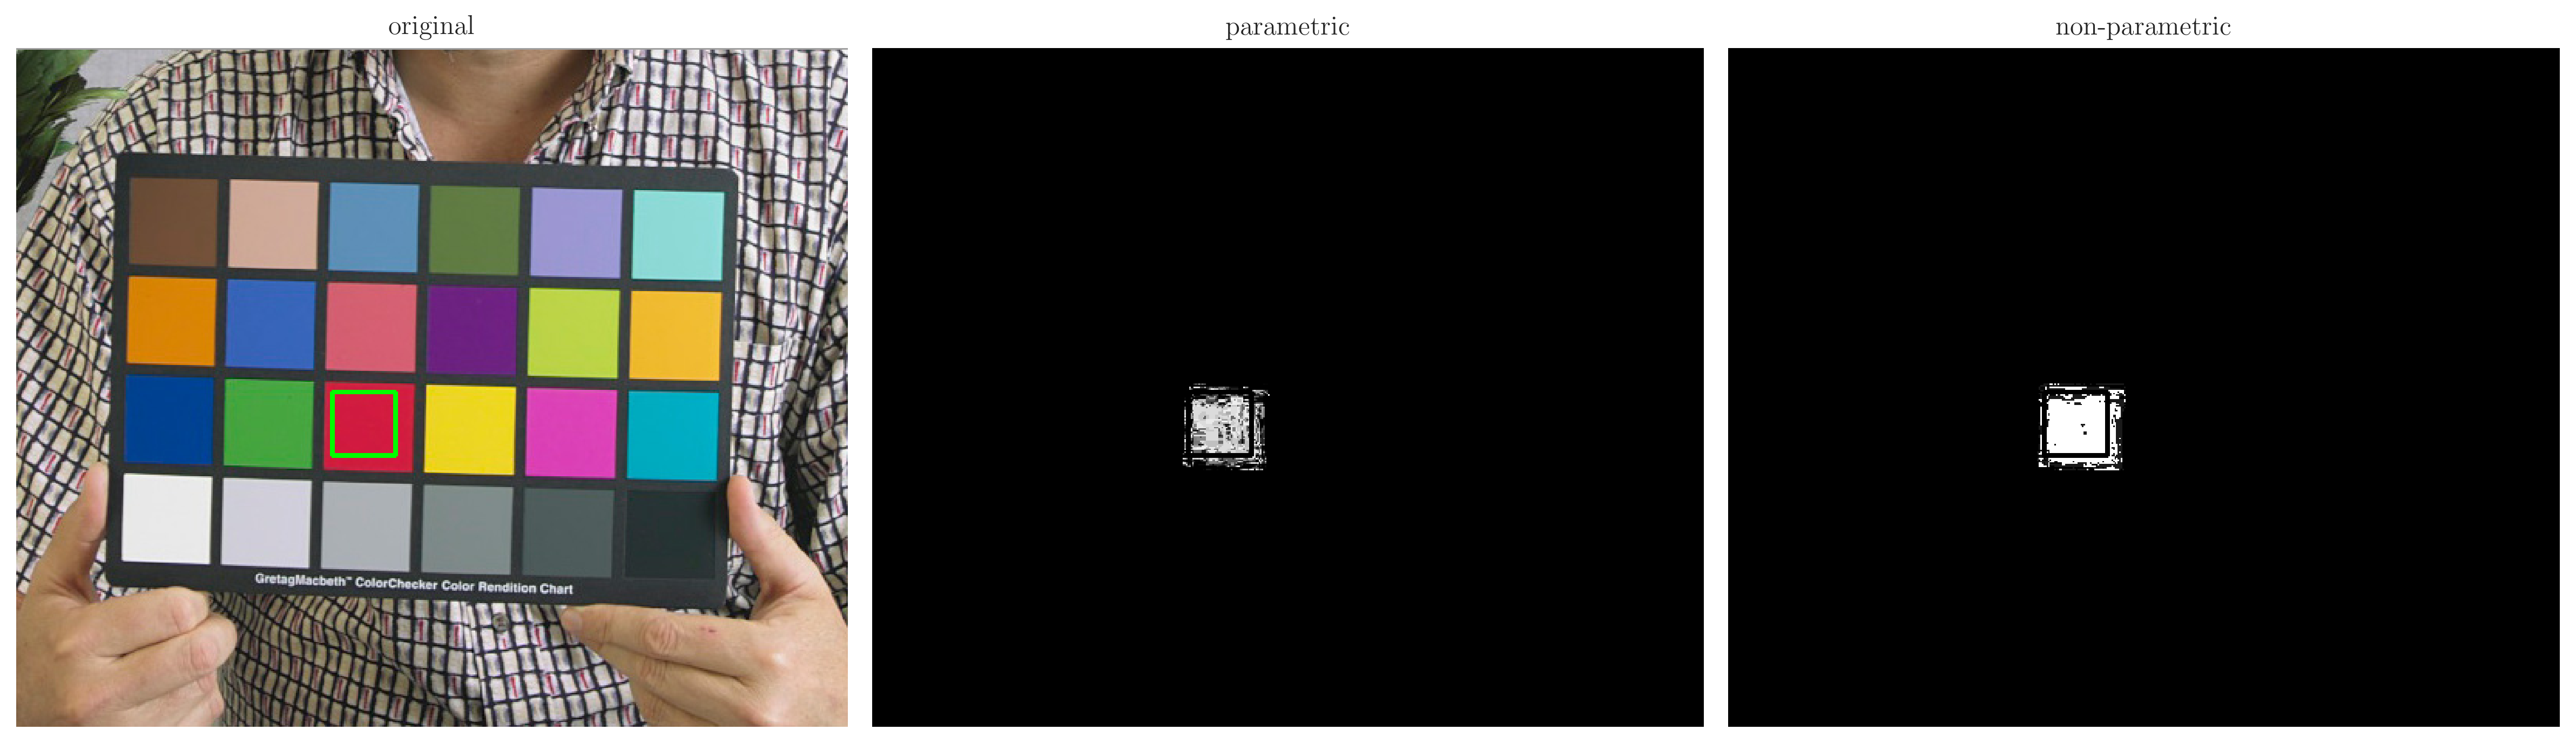
\includegraphics[width=\textwidth]{mac_red_out.png}
	\caption{A Macbeth ColorChecker (left) and the output from parametric (middle) and non-parametric (right) algorithms. The specific region of interest is the bright green box outlining a portion of the red patch. Both algorithms segment the ROI pretty well, with the non-parametric algorithm appearing to be more sensitive.}
	\label{fig:macbeth-red}
\end{figure}

\begin{figure}[htb]
	\centering
	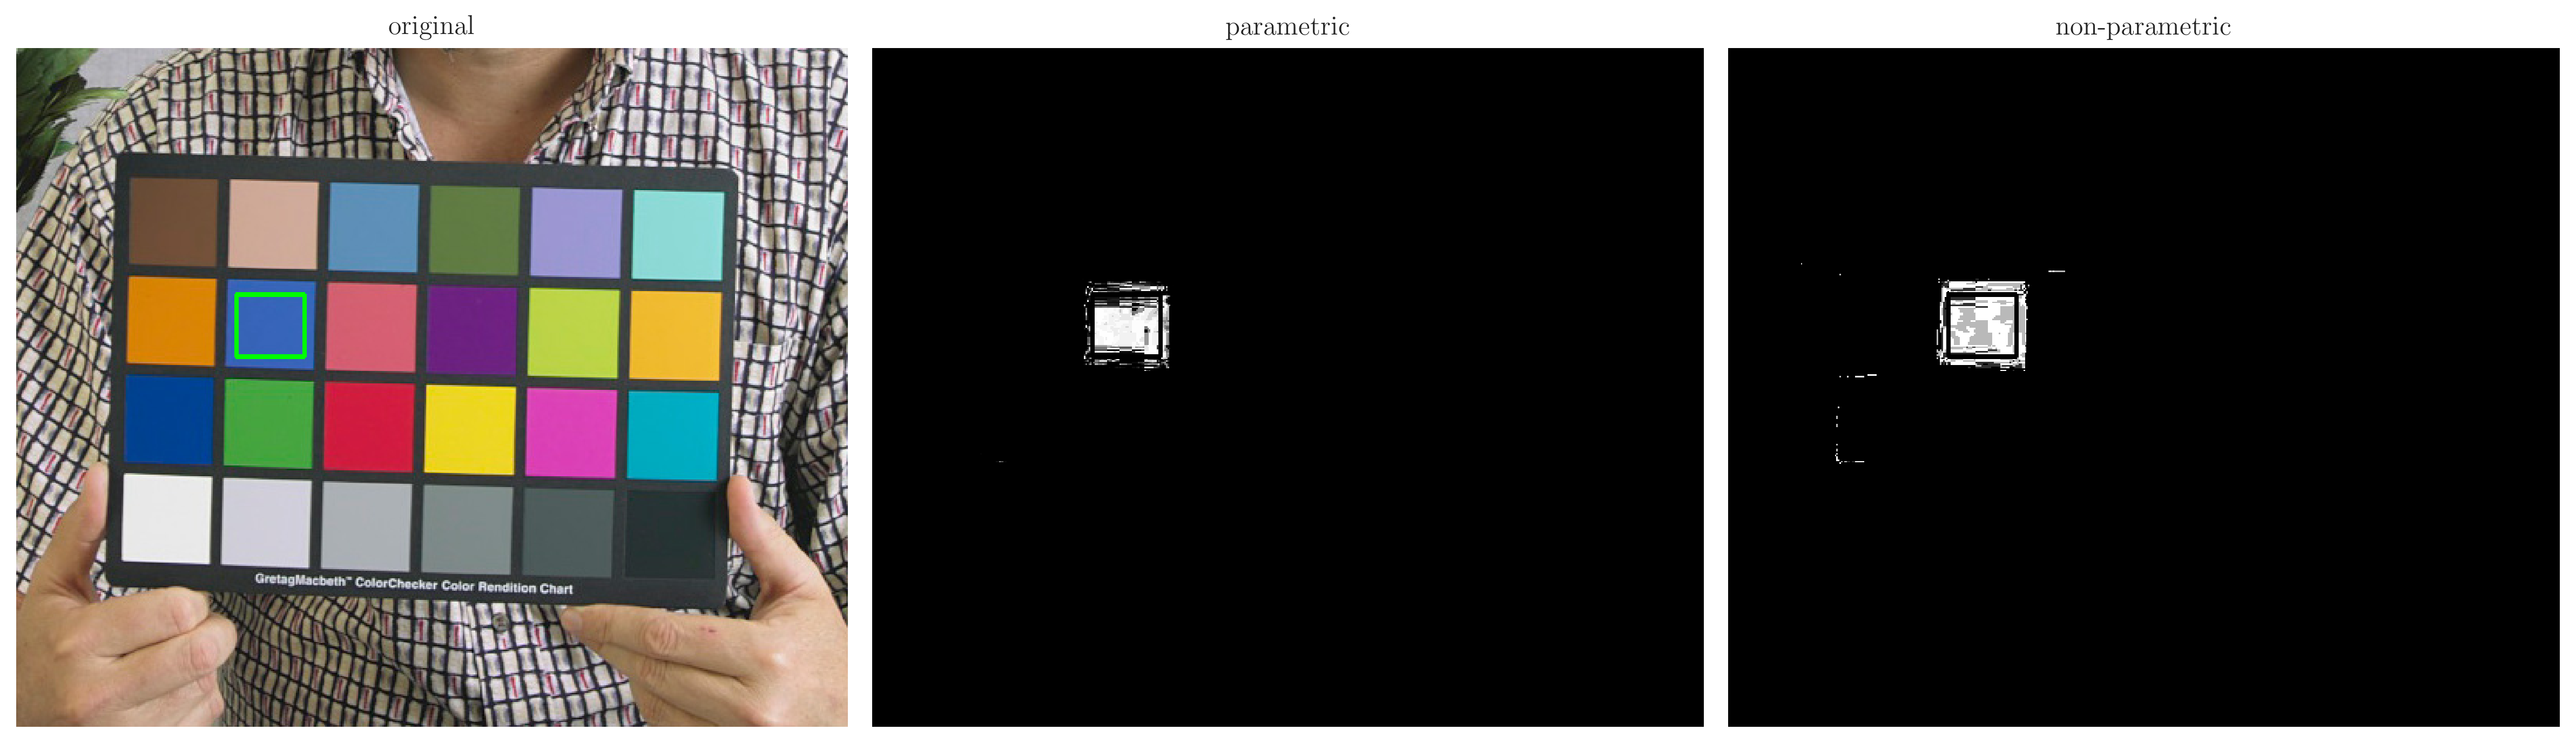
\includegraphics[width=\textwidth]{mac_blue_out.png}
	\caption{Macbeth ColorChecker (left) parametric output (middle) and non-parametric output (right). The specific ROI is the bright green box outlining a portion of the middle blue patch. The parametric algorithm keeps the segmentation confined to the concerned patch, while the non-parametric algorithm is slightly detecting a portion of the other blue patches at the ROI's lower-left and upper-right corners.}
	\label{fig:macbeth-blue}
\end{figure}

\begin{figure}[htb]
	\centering
	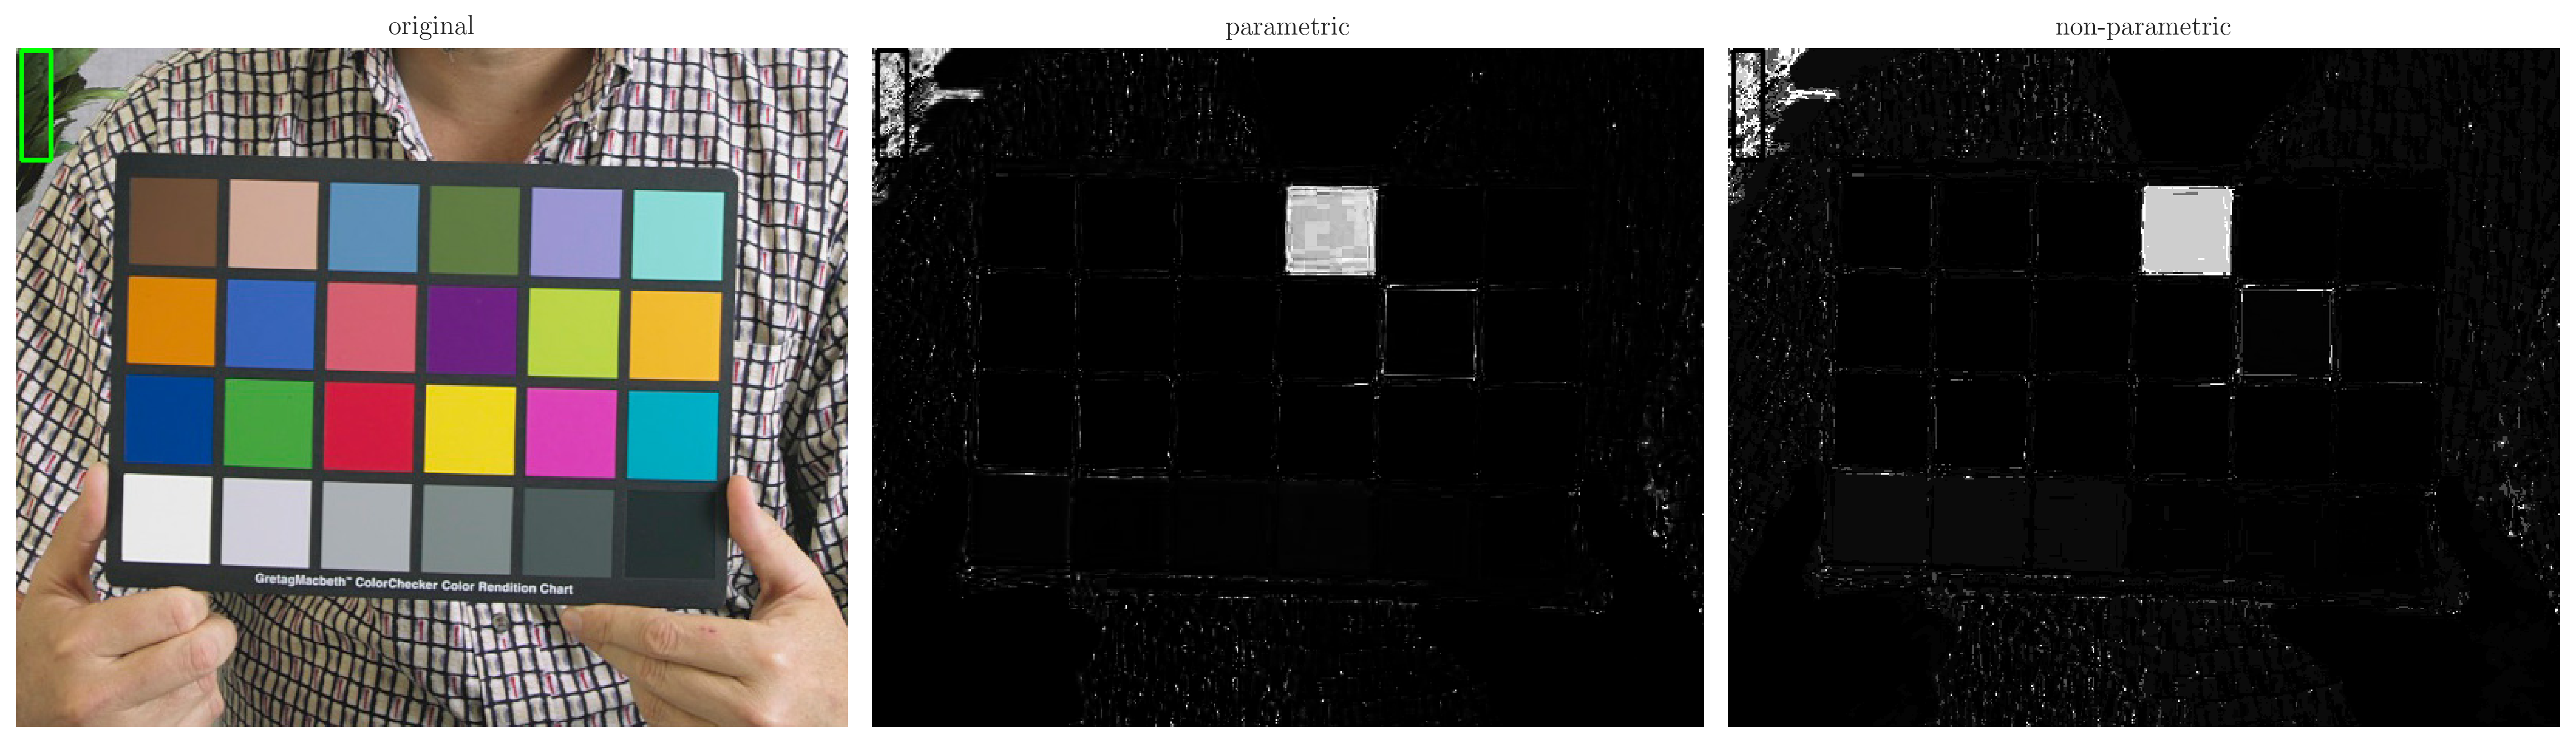
\includegraphics[width=\textwidth]{mac_green_out.png}
	\caption{Macbeth ColorChecker (left) parametric output (middle) and non-parametric output (right). The specific ROI is the bright green box outlining the plant on the upper left corner. Both algorithms segmented not only the plant, but also the olive-green patch, as well as some portions on the person's clothes. Closer examination of the original image shows that there are some green reflections off the clothes, suggesting the imaging location is surrounded by a few plants.}
	\label{fig:macbeth-green}
\end{figure}

\begin{figure}[htb]
	\centering
	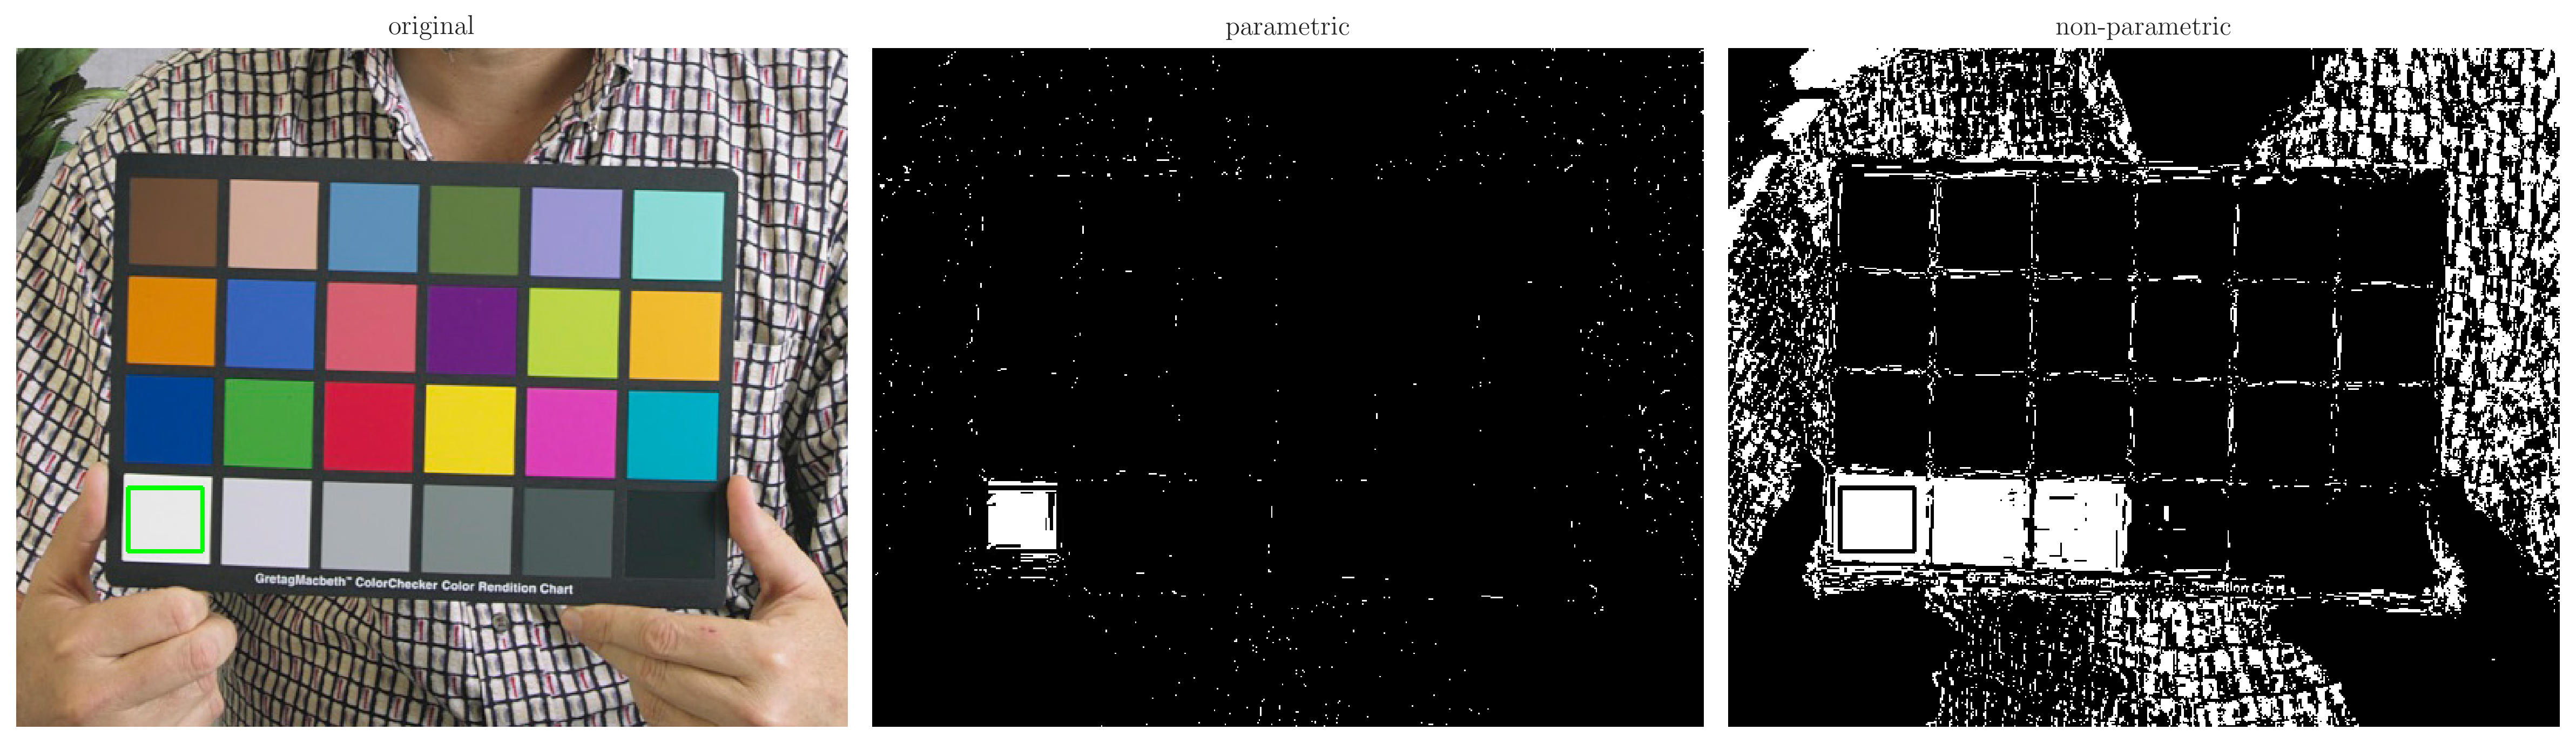
\includegraphics[width=\textwidth]{mac_white_out.png}
	\caption{Macbeth ColorChecker (left) parametric output (middle) and non-parametric output (right). The specific ROI is the bright green box outlining the white patch. The parametric algorithm better confines the segmented area to the white patch, while the non-parametric algorithm segmented the white patch along with the two adjacent gray patches and the person's clothes (which is also generally white).}
	\label{fig:macbeth-white}
\end{figure}

\begin{figure}[htb]
	\centering
	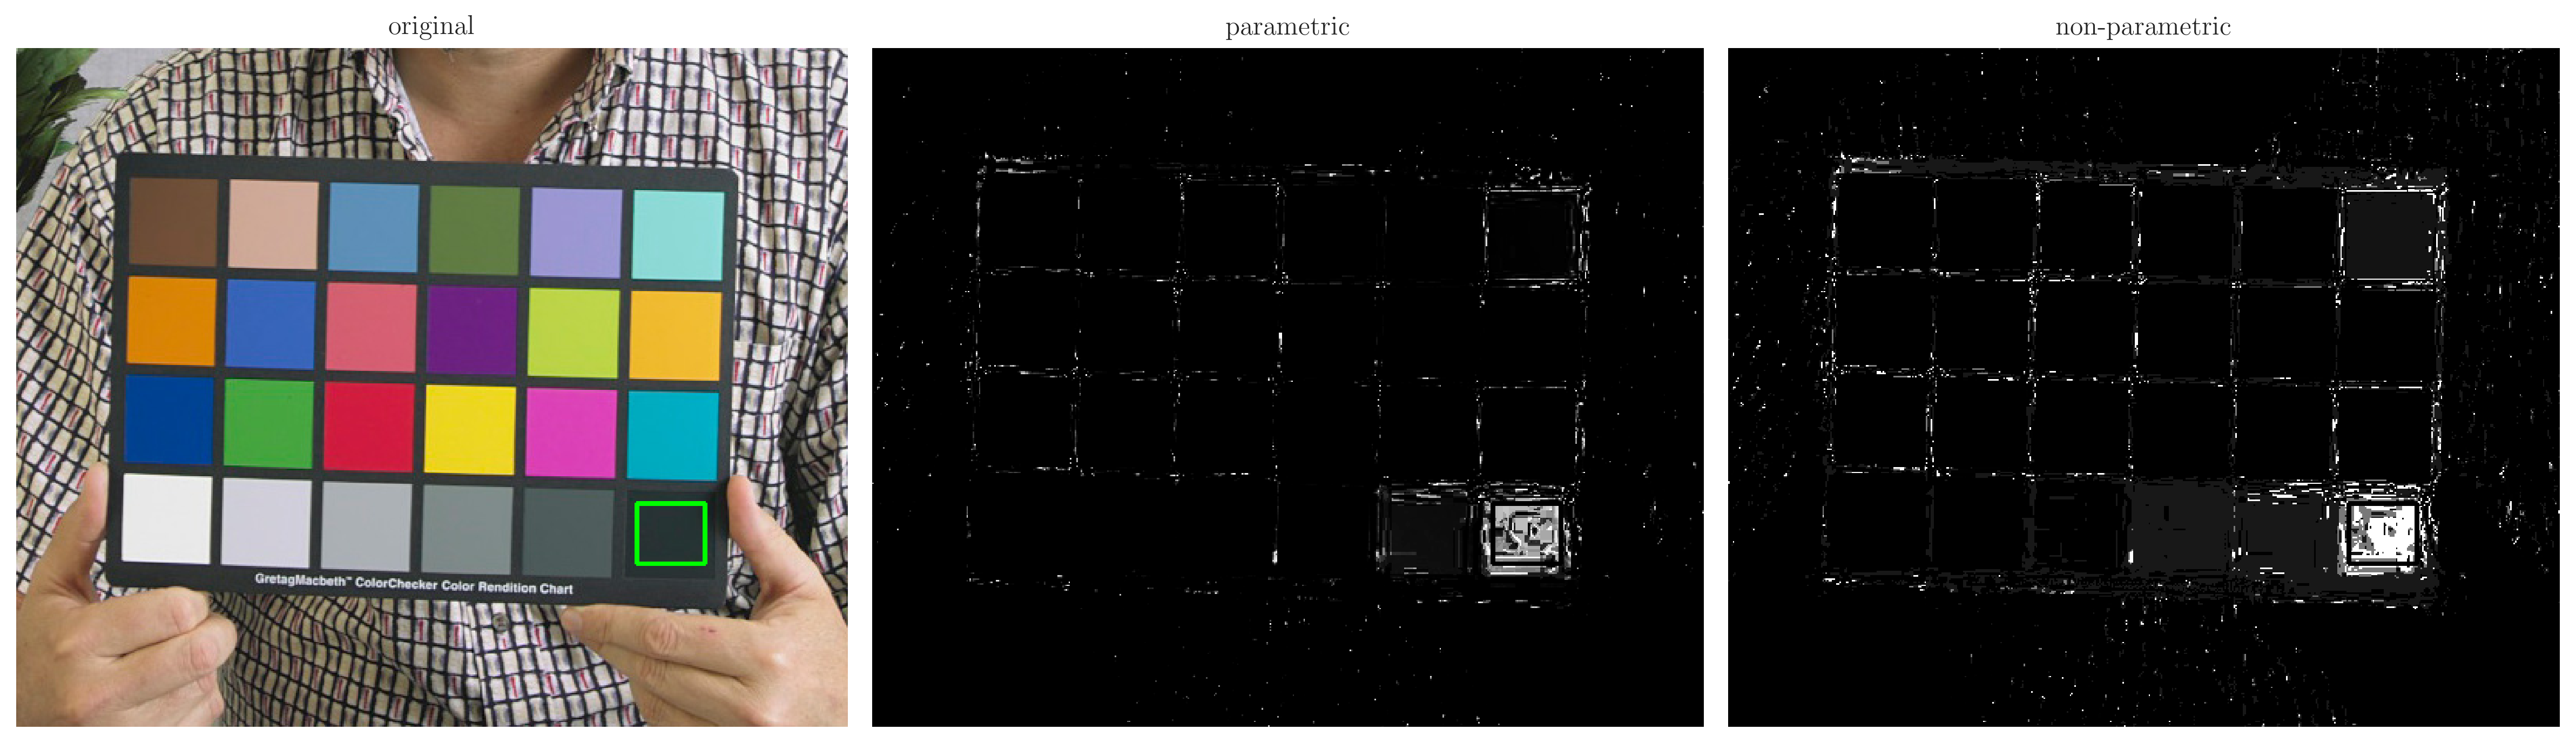
\includegraphics[width=\textwidth]{mac_black_out.png}
	\caption{Macbeth ColorChecker (left) parametric output (middle) and non-parametric output (right). The specific ROI is the bright green box outlining a portion of the black patch. Both algorithms segment the black patch along with the ColorChecker's borders and portions of the adjacent gray patches.}
	\label{fig:macbeth-black}
\end{figure}

\clearpage
\subsection{Implementation: Skin}
To realize these methods' effectivity in a more practical situation, let's try applying them to images with more chromatic and luminant variety. I'll be using a fairly simple portrait which has a well-defined background and foreground, taken with natural light, and I'll try to segment only the skin. Let's call the image Jena (used with her permission). Note that the image has already been post-processed, meaning white balance corrections, contrast adjustments, exposure corrections, and artistic color grading have all been applied. As a human observer, the separation between foreground and background is pretty clear-cut. However, we can expect a machine to have some problems because the color of Jena's shirt is quite close to the color of her skin and to the background. Notice also that due to direct sunlight, there is a lot of specular reflection on her face and hands. Also, due to the image being taken at high ISO (around 400, to account for the fast shutter speed used in order for the confetti not to blur, and the considerably narrow aperture used in order for as much of the elements to be in focus as possible), we can observe some visible grain in the shadows, particularly on the side of her right forearm facing away from the light. Figures \ref{fig:jena-arm}--\ref{fig:jena-forehead} show the results of varying the location of the ROI.

We can observe that although parametric segmentation seems to work best in the Macbeth trial, non-parametric segmentation seems to work consistently better when it comes to practical images because pixel values are rarely normally distributed about the mean.


\begin{figure}[htb]
	\centering
	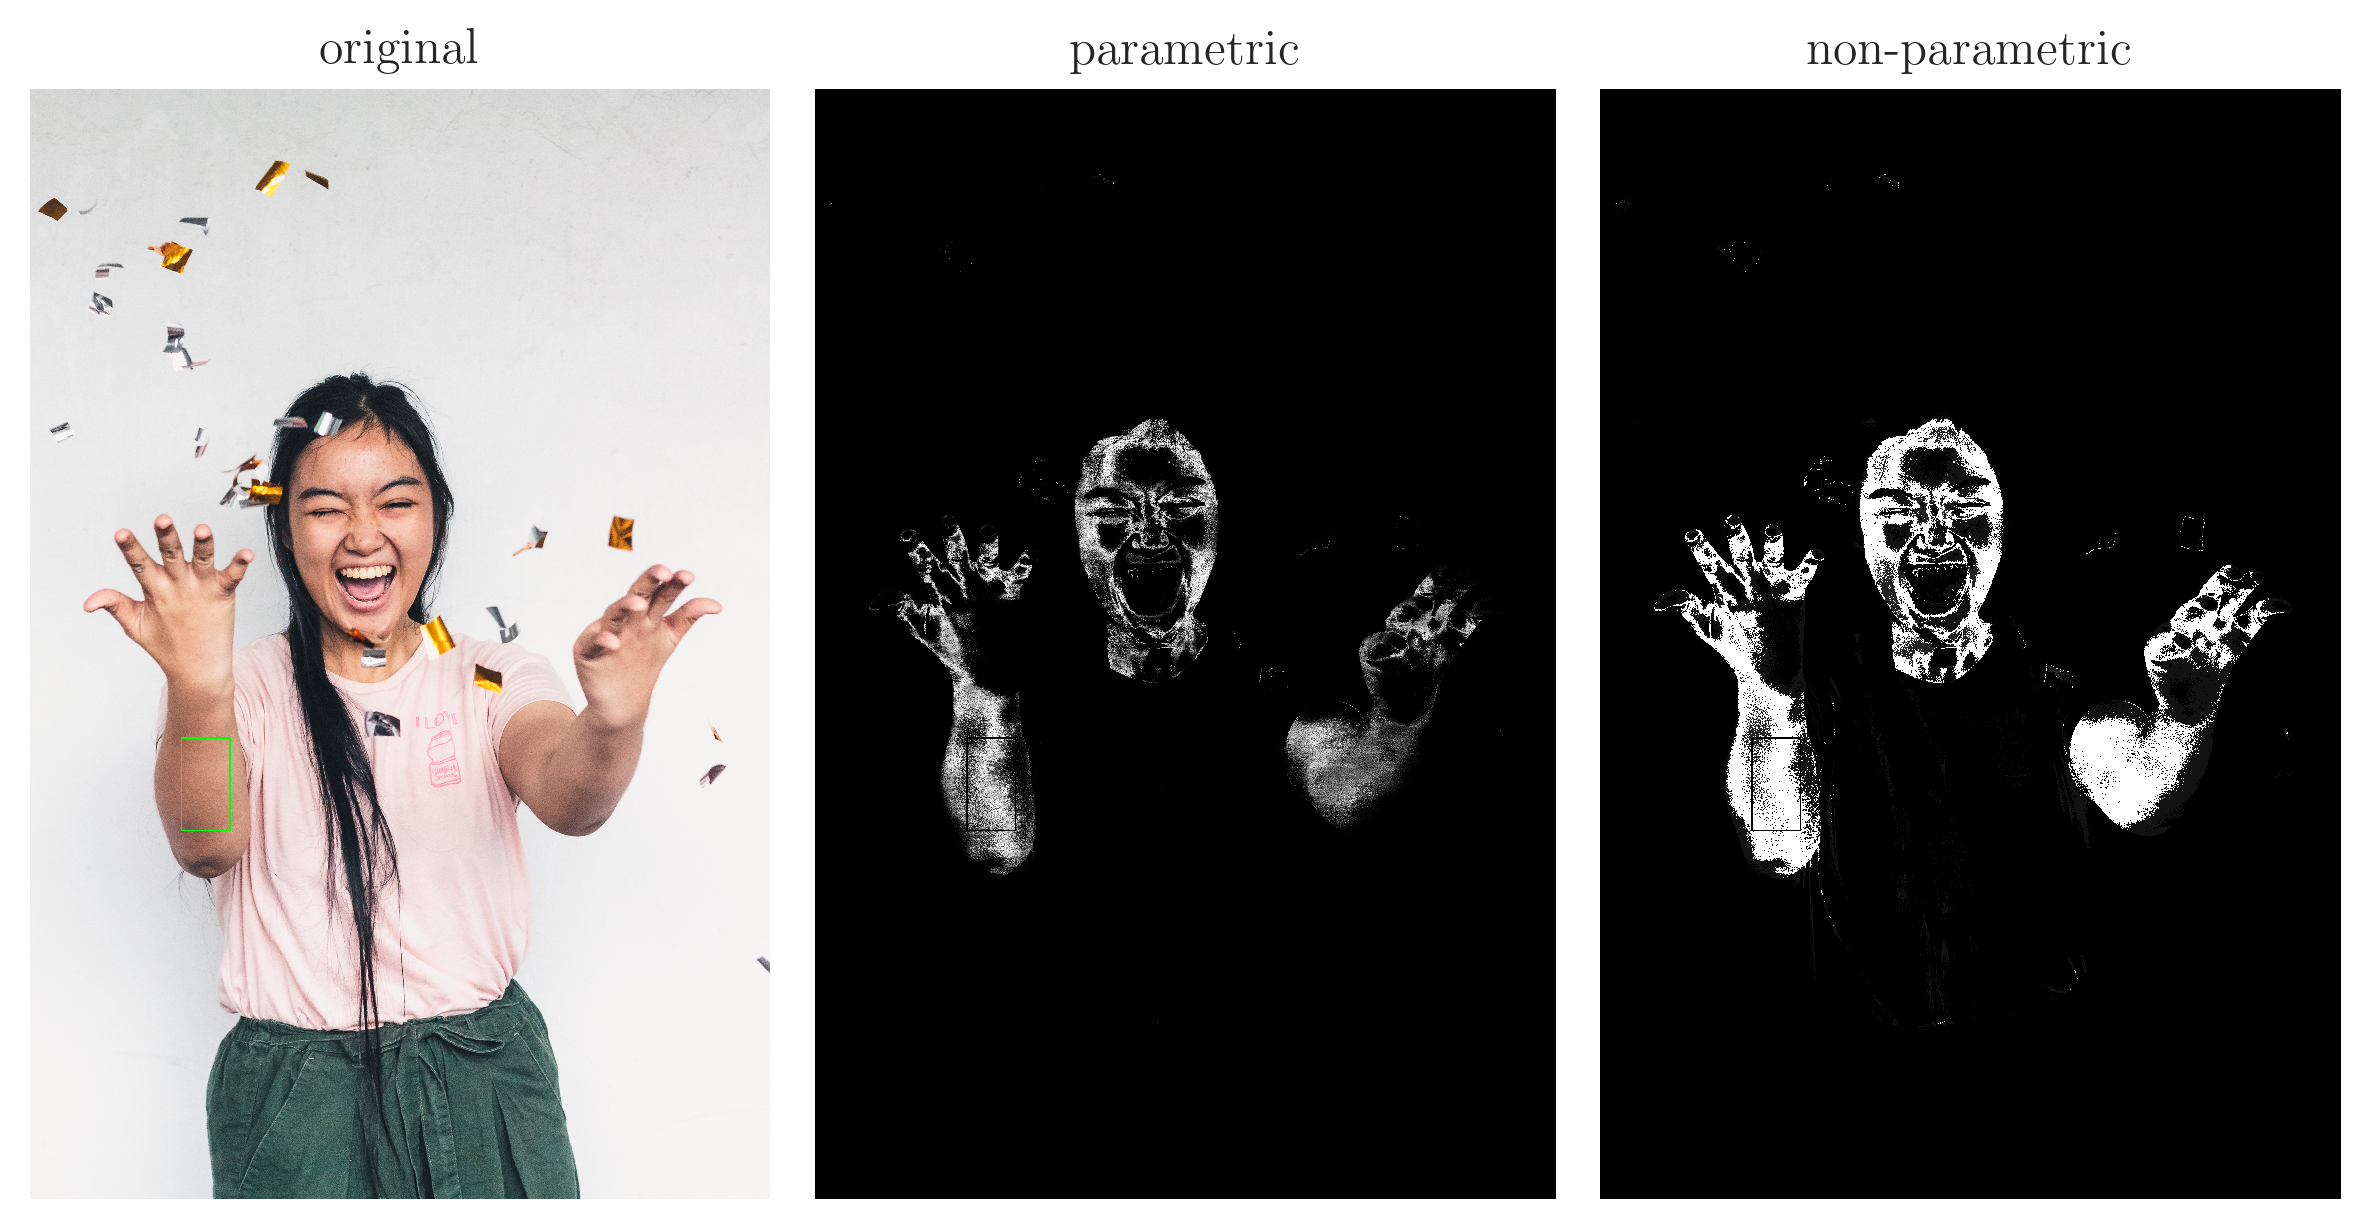
\includegraphics[width=\textwidth]{jena_arm_out.png}
	\caption{Jena (left) parametric output (middle) and non-parametric output (right). The specific ROI is the bright green box outlining a portion of her right forearm. This first attempt was quite good. Again, non-parametric appears to be more sensitive, but both of them fail to account for the regions of the skin with high specular reflection.}
	\label{fig:jena-arm}
\end{figure}

\begin{figure}[htb]
	\centering
	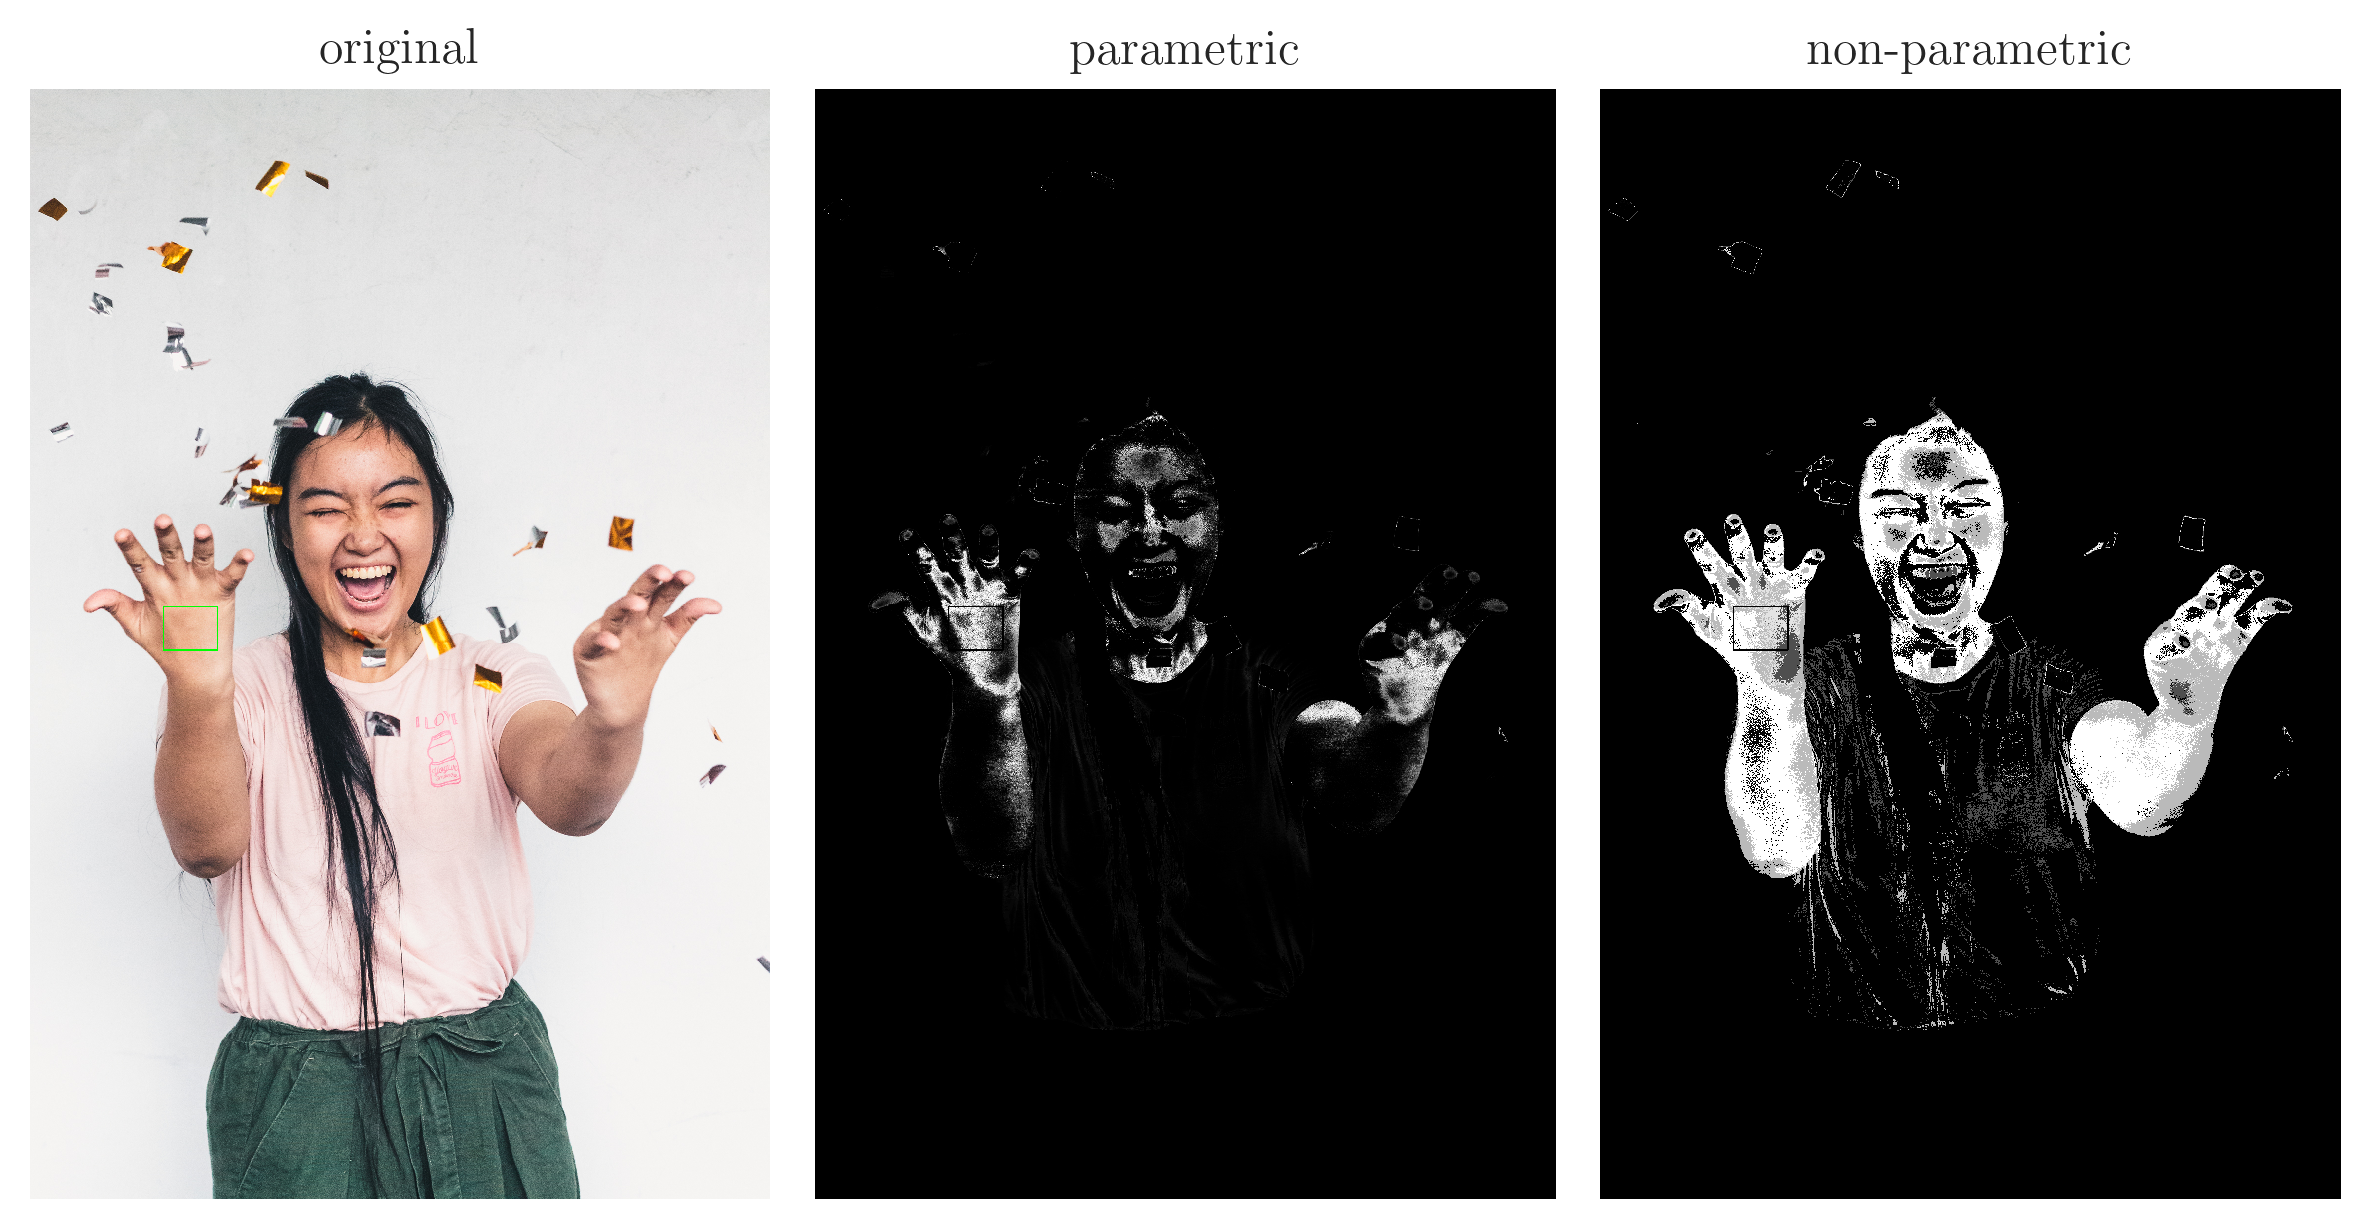
\includegraphics[width=\textwidth]{jena_hand_out.png}
	\caption{Jena (left) parametric output (middle) and non-parametric output (right). The specific ROI is the bright green box outlining a portion of her right hand. Once again, non-parametric wins this one as more of the specular regions have been segmented. However, this comes at a cost of segmenting some of the creases on her shirt. The parametric method performs quite poorly as less of the skin has been segmented as compared to Fig. \ref{fig:jena-arm}.}
	\label{fig:jena-hand}
\end{figure}

\begin{figure}[htb]
	\centering
	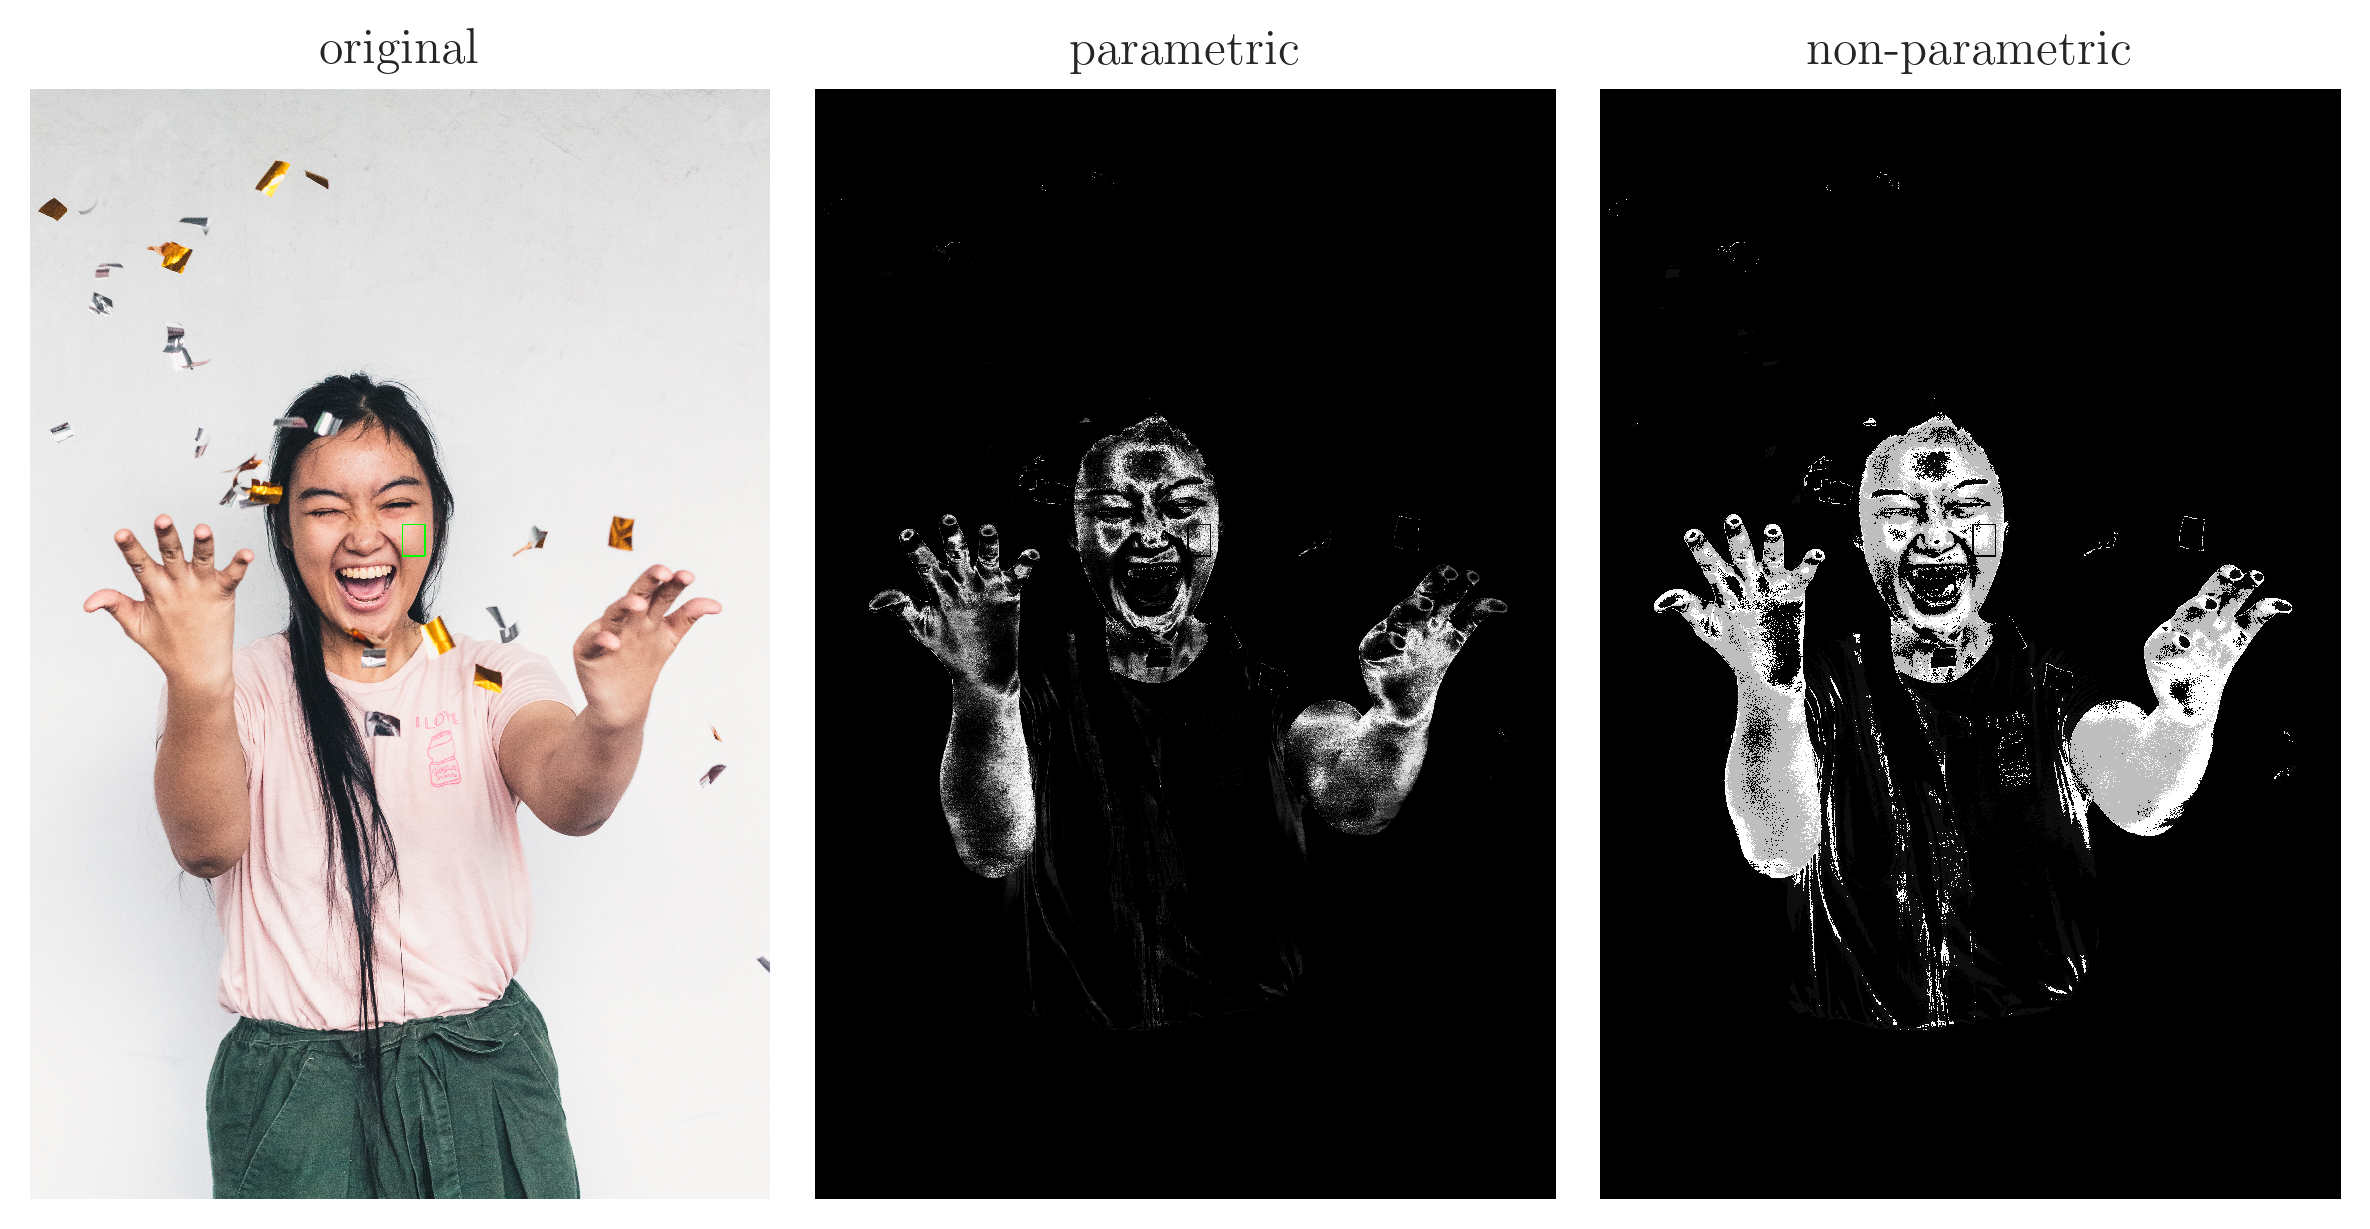
\includegraphics[width=\textwidth]{jena_cheek_out.png}
	\caption{Jena (left) parametric output (middle) and non-parametric output (right). The specific ROI is the bright green box outlining a portion of her left cheek. Once again, we can observe an improvement in non-parametric segmentation, while parametric segmentation got worse. The non-parametric method was able to segment even more of the regions with high intensity specular reflection, but again, at the cost of segmenting more of the shirt due to their similarity in color.}
	\label{fig:jena-cheek}
\end{figure}

\begin{figure}[htb]
	\centering
	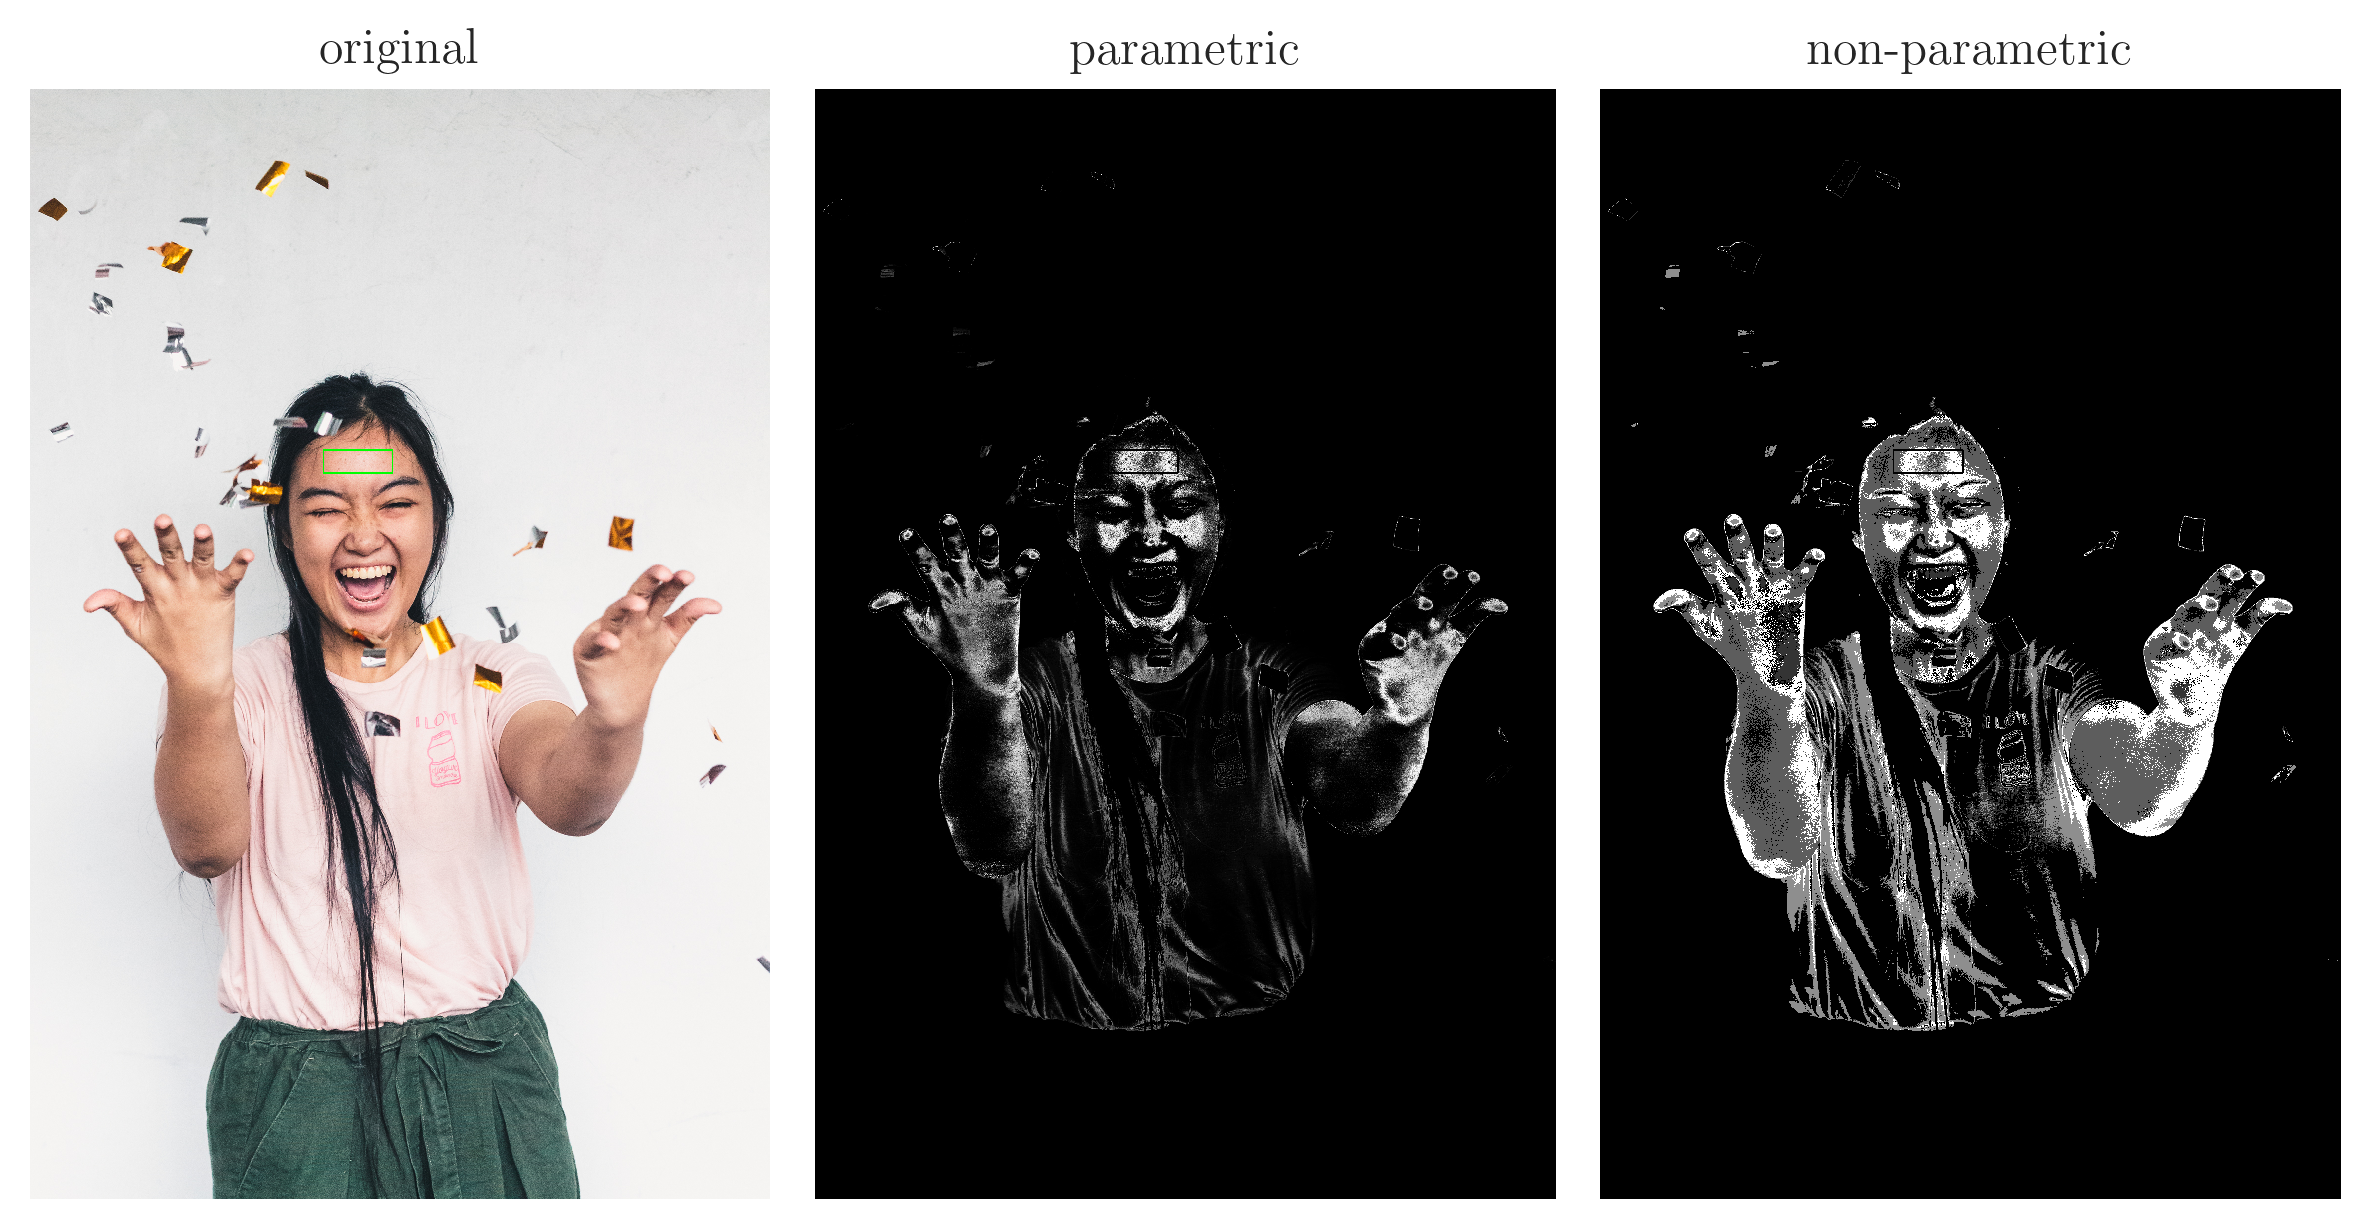
\includegraphics[width=\textwidth]{jena_forehead_out.png}
	\caption{Jena (left) parametric output (middle) and non-parametric output (right). The specific ROI is the bright green box outlining a portion of her forehead. This one was able to segment the most skin out of all the sampling ROIs, but also segmented a lot of unwanted pixels. This is because we have captured some of the specular reflection, whose color closely matches that of the background and the shirt.}
	\label{fig:jena-forehead}
\end{figure}

\clearpage
\subsection*{Implementation: Cancer cells}
For the last application we'll try segmenting a sample of red blood cells with acute lymphoma, sourced from \cite{cancer}, using everything we've discussed so far. The original image along with its parametric and non-parametric segmentation outputs are shown in Fig. \ref{fig:cancer}, while the output from Otsu's method is in Fig. \ref{fig:cancer-otsu}. The reason we are applying Otsu's method for this image and not for the Macbeth or Jena images is because we have a clear-cut foreground and background in this image. The Macbeth image contains too many different patches of different colors, so its histogram is hardly bimodal. The Jena image does have a separable foreground/background, but what we want to segment is the skin, not the foreground; Otsu's method will most likely segment Jena's entire body.

\begin{figure}[htb]
	\centering
	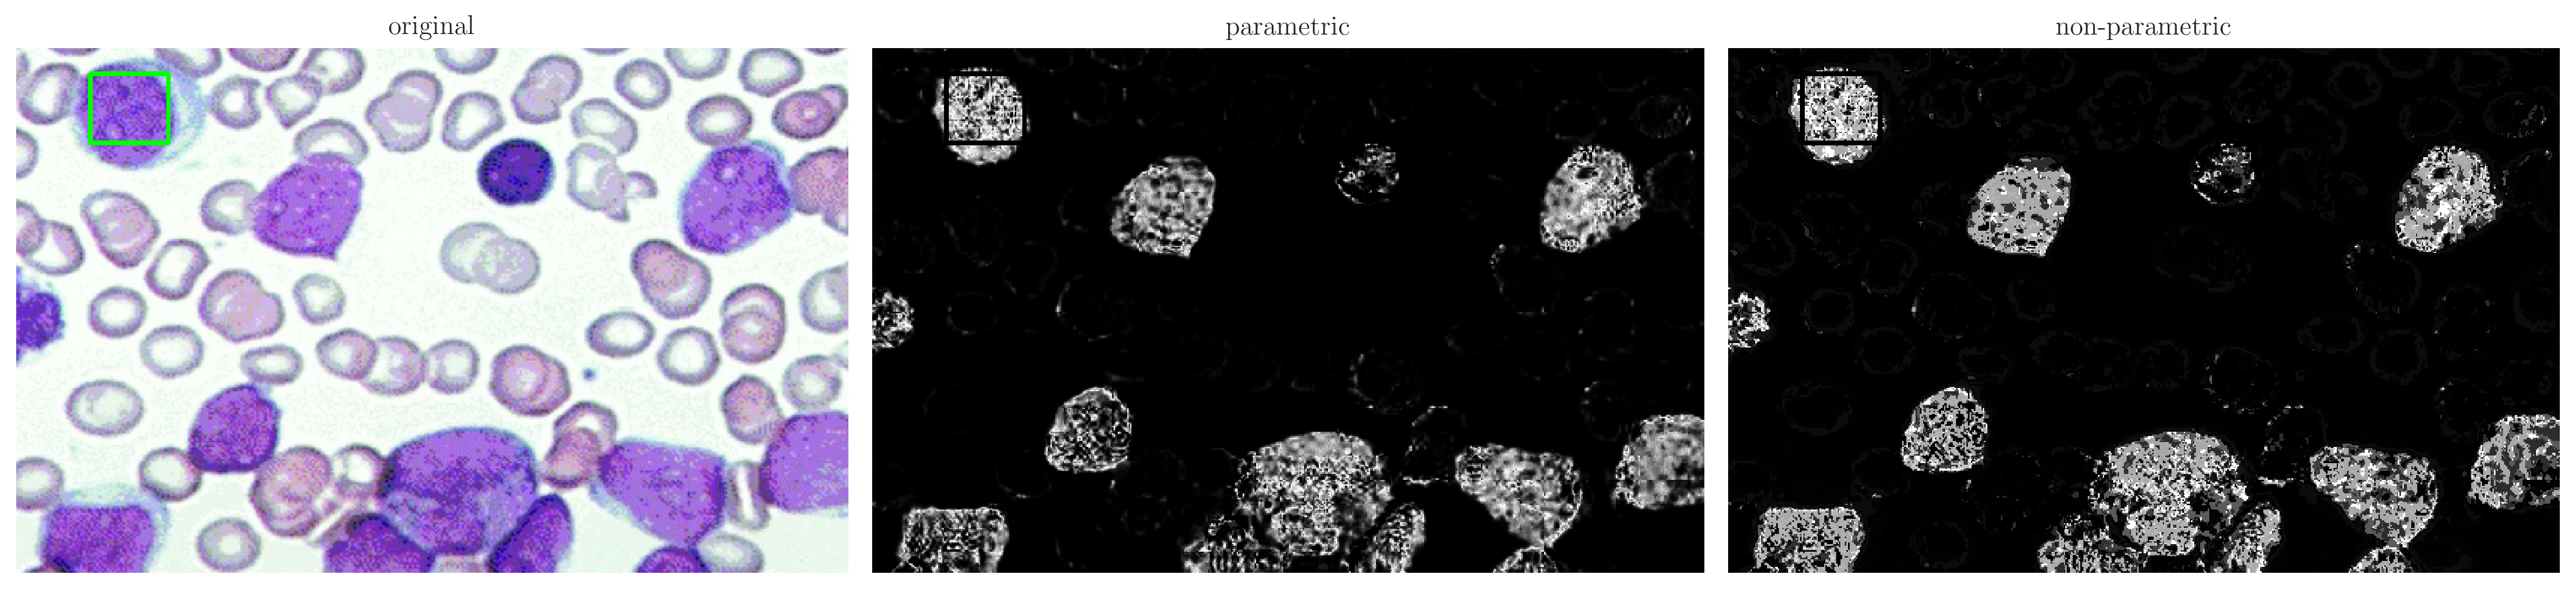
\includegraphics[width=\textwidth]{cancer_giemsa.png}
	\caption{Healthy and cancerous red blood cells (left) parametric output (middle) and non-parametric output (right). The specific ROI is the bright green box outlining a portion of a giemsa-stained cancerous cell on the top left corner. Notice that both methods perform similarly and manage to capture only the stained cells.}
	\label{fig:cancer}
\end{figure}

\begin{figure}[htb]
	\centering
	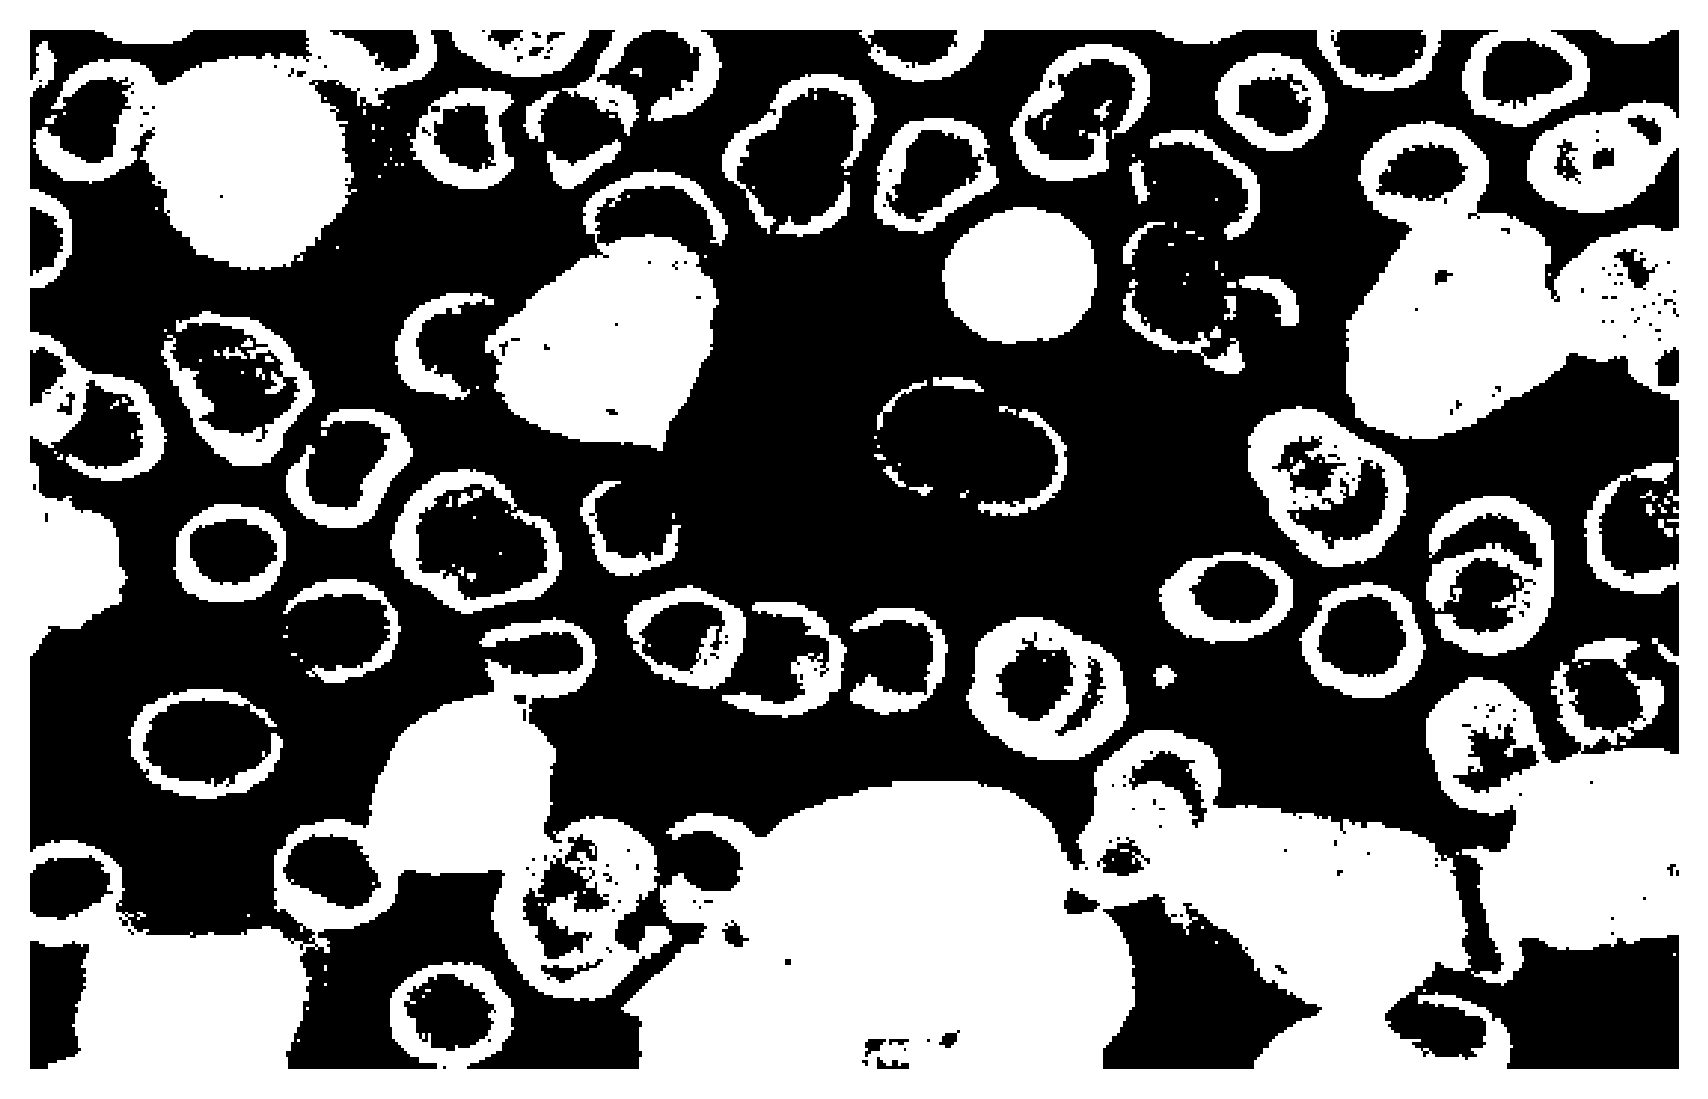
\includegraphics[width=0.5\textwidth]{cancer_otsu.png}
	\caption{Cancer cell segmentation via Otsu's method. At first glance, this does method does not seem to be appropriate as it segments all the cells. However, according to \cite{malaria}, healthy RBCs can be characterized as hollow, torus-like shapes when they are Otsu-thresholded; if a significant amount of the RBC's nucleus is segmented, that could indicate something wrong with the cell. In the image, we can see that the cancerous cells are completely segmented, so we can say from this interpretation that Otsu's method is a valid segmentation algorithm for applications such as this.}
	\label{fig:cancer-otsu}
\end{figure}

\clearpage
\begin{table}[!htb]
	\centering
	\caption{Self-evaluation.}
	\begin{tabular}{||r|c||}
		\hline
		Technical correctness & 5 \\ \hline
		Quality of presentation & 5 \\ \hline
		Initiative & 2 \\ \hline
		\textbf{TOTAL} & \textbf{12} \\ \hline
	\end{tabular}
	\label{tab:self-eval}
\end{table}

\bibliographystyle{spp-bst}
\bibliography{186-Act7}

\end{document}